Um ein Bild von der allgemeinen Übereinstimmung der simulierten Daten mit den tatsächlich beobachteten Daten zu erhalten, wird in diesem Kapitel das Jahresmittel der simulierten und beobachteten Daten verglichen. Dadurch erhält man einen Überblick über die geographische Übereinstimmung der Regenzonen und Trockengebiete im abgebildeten Bereich.
\section{Herangehensweise}
\begin{enumerate}
	\item Berechnung des jährlichen Mittelwertes pro Gitterzelle über aller Jahre.
	\item Subtraktion dieser Mittelwerte (Simuliert - Beobachtet).	
\end{enumerate}
\section{Mittlerer Bias}
In diesem Unterkapitel soll das Verhalten der gemittelten Differenzen aller Datensätze aufgezeigt werden.\\
Wie man gut in den Abbildungen \ref{fig:mean_boxplots} erkennen kann, liegt die Abweichung der Evaluation-Datensätze weit näher bei 0, als die in den Historical-Datensätzen. Des Weiteren ist gut zu erkennen, dass die Abweichung des Datensatzes ALP-3 betrieben mit den Re-Analysedaten (Evaluation) die Beobachtungsdaten gut abbildet und somit im Mittel ein relativ gutes Klimamodell für den Alpenraum darstellt.
Beide Klimamodelle, betrieben mit dem GCM MPI-ESM-LR (Hisorical), liefern Ergebnisse, die eine starke Abweichung in positive Richtung aufweisen, wobei sie sich nur mehr in der Stärke der Ausreißer unterscheiden: Das CCLM5-0-9 hat weitaus stärkere Ausreißer. Die Abbildungen zeigen, dass im Mittel zwar die Ausreißer des regionalem Klimamodells CCLM5-0-9 im Gegensatz zum CCLM4-8-17 stärker sind, jedoch sich der Bias kaum unterscheidet. Im Mittel ist also die Vorhersagequalität der beiden Modelle nahezu identisch. Man kann auch beim Vergleichen der beiden Evaluation-Datensätze mit den beiden Historical-Datensätzen erkennen, dass das globale Klimamodell im Alpenraum den Niederschlag zu stark simuliert, was den ins Positive verschobenen Bias erklärt.\\
Da sich diese Abweichungen nicht über das gesamte Gitter gleich abzeichnen, wird in Folge auf die geographische Verteilung der Abweichungen eingegangen.

\begin{figure}[h!]
	\begin{subfigure}{0.49\textwidth}
		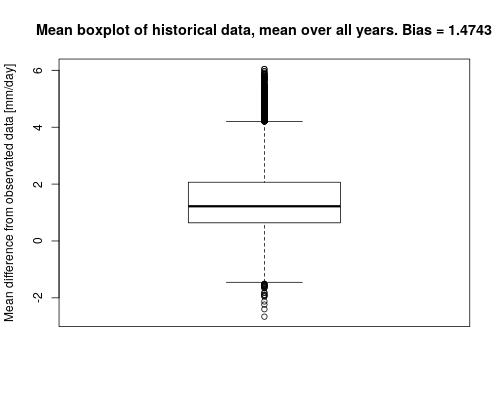
\includegraphics[width=\textwidth]{mean_n/eur_11_mean_historical_boxplot.jpg}
		\caption{Historical, EUR-11}
	\end{subfigure}
	\begin{subfigure}{0.49\textwidth}
		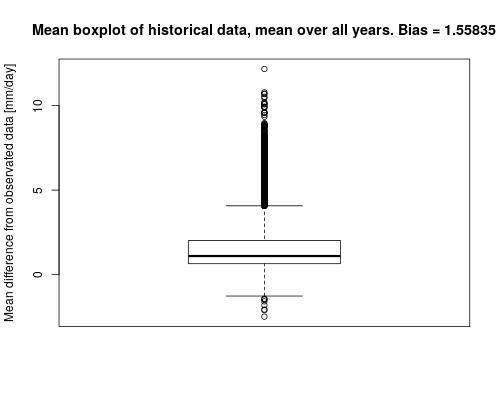
\includegraphics[width=\textwidth]{mean_n/alp3_mean_historical_boxplot.jpg}
		\caption{Historical, ALP-3}
	\end{subfigure}
	\begin{subfigure}{0.49\textwidth}
		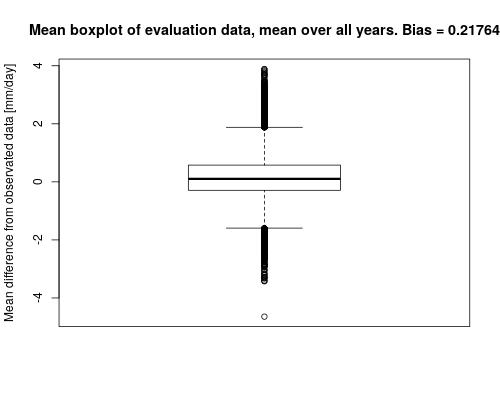
\includegraphics[width=\textwidth]{mean_n/eur_11_mean_evaluation_boxplot.jpg}
		\caption{Evaluation, EUR-11}
	\end{subfigure}
	\begin{subfigure}{0.49\textwidth}
		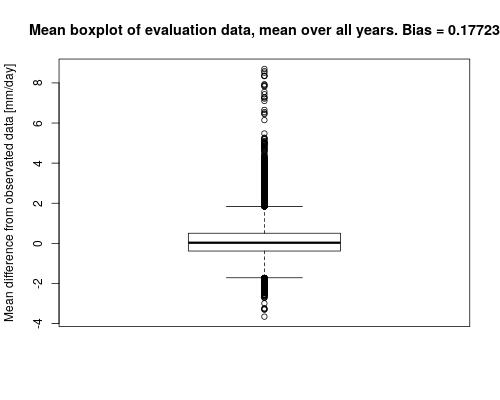
\includegraphics[width=\textwidth]{mean_n/alp3_mean_evaluation_boxplot.jpg}
		\caption{Evaluation, ALP-3}
	\end{subfigure}
	\caption{Box-Plots der Differenzen des jährlichen Mittels des Niederschlags. (gemittelt über alle Jahre)}
	\label{fig:mean_boxplots}
\end{figure}


\begin{figure}[h!]
	\begin{subfigure}{0.49\textwidth}
		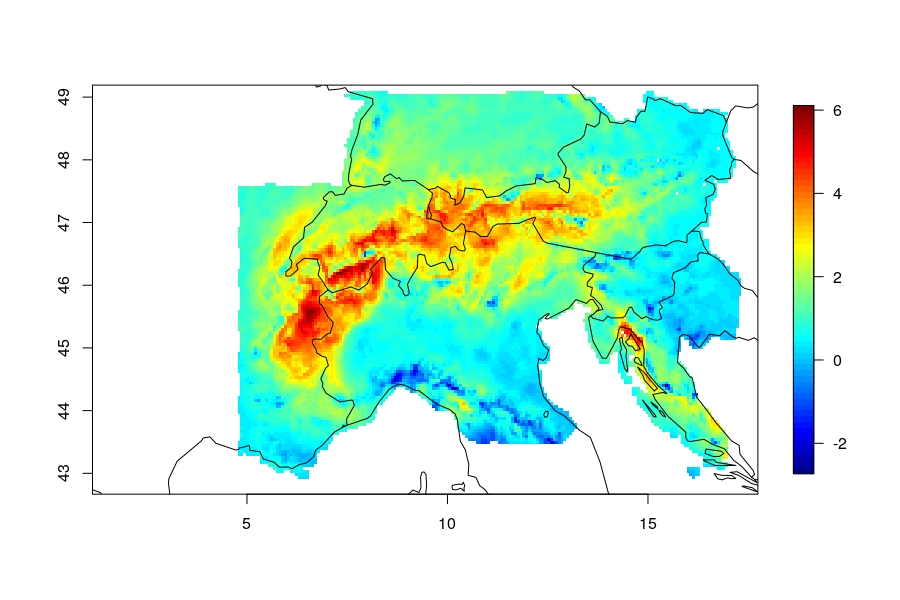
\includegraphics[width=\textwidth]{mean_n/mean_diff_hist_eur11.jpeg}
		\caption{Historical, EUR-11}
	\end{subfigure}
	\begin{subfigure}{0.49\textwidth}
		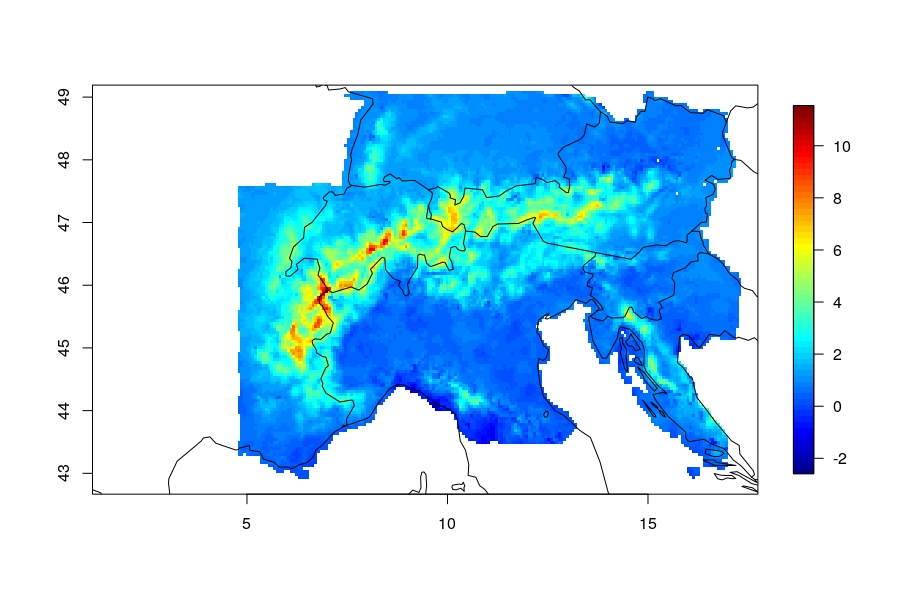
\includegraphics[width=\textwidth]{mean_n/mean_diff_hist_alp3.jpeg}
		\caption{Historical, ALP-3}
	\end{subfigure}
	\begin{subfigure}{0.49\textwidth}
		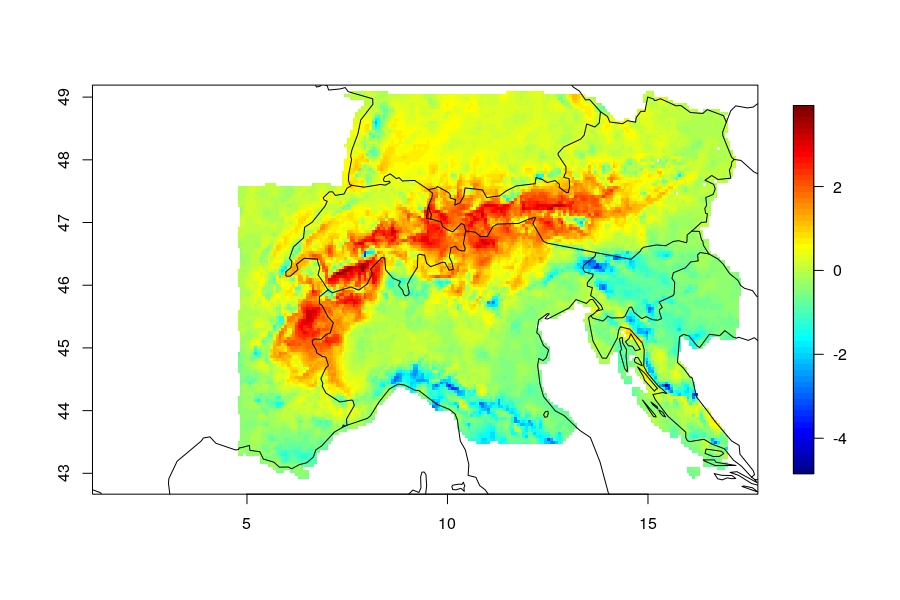
\includegraphics[width=\textwidth]{mean_n/mean_diff_eval_eur11.jpeg}
		\caption{Evaluation, EUR-11}
	\end{subfigure}
	\begin{subfigure}{0.49\textwidth}
		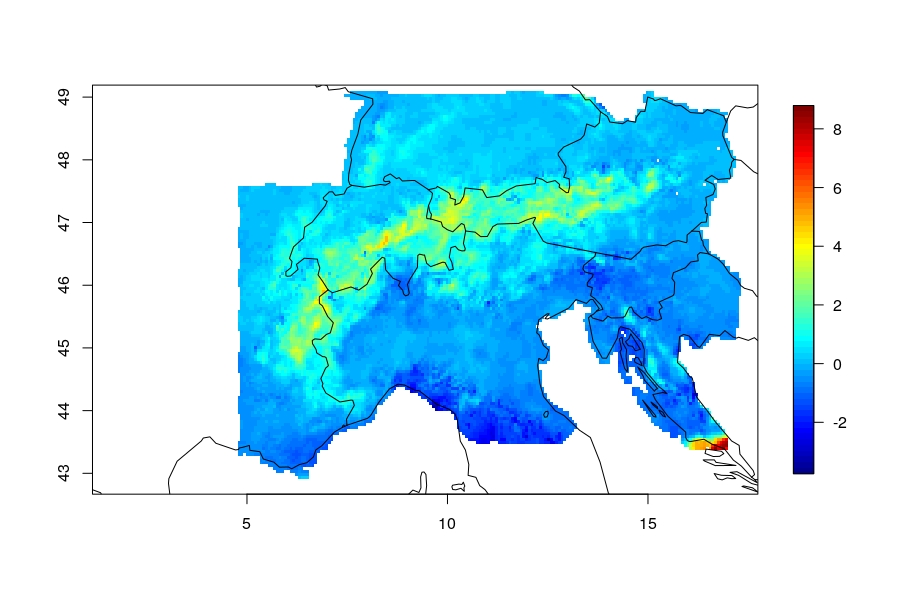
\includegraphics[width=\textwidth]{mean_n/mean_diff_eval_alp3.jpeg}
		\caption{Evaluation, ALP-3}
	\end{subfigure}
	\caption{Geographische Verteilung der Differenzen (Modell-Beobachtungsdaten) vom jährlichen Mittel des Niederschlags [mm/Tag] gemittelt über alle Jahre}
	\label{fig:mean_diff}
\end{figure}

Die geographische Verteilung der Abweichungen wurden in Abb. \ref{fig:mean_diff} für alle Datensätze dargestellt. Man erkennt gut, dass sich die größten Abweichungen an den Gebirgskämmen abzeichnen. Über den orthographisch gediegenen Gegenden ist die Abweichung vom Beobachtungsdatensatz relativ gering. Das hat den Grund, dass sich in gebirgigen Gegenden  kleinen Konvektionszellen bilden, die sich zu größeren Regenzellen aufschaukeln können. Das gröber aufgelöste Modell CCLM4-8-17, mit einer Auflösung von ungefähr 15km, kann diese Wettererscheinungen nicht modellieren - viele Täler in diesen Gegenden sind schmäler als 15km. Sie sind nur durch die parametrisierte Konvektion darstellbar. Dieses Modell scheint durch sein höheres Alter bereits feiner getuned geworden zu sein, als das Verglichene CCLM5-0-9: Die Abweichungen überschreiten kaum 6 mm/Tag, wie auch schon in der Abbildung \ref{fig:mean_boxplots} dargestellt ist.\\
Das feiner aufgelöste regionale Klimamodell CCLM5-0-9 (ALP3) müsste in diesen Gegenden einen klaren Vorteil haben, da die Konvektion dynamisch simuliert wird. Jedoch scheinen die Gleichungen bzw. die einzelnen Module des Modells noch nicht hinreichend abgestimmt (getuned) worden zu sein.\\
Ein im Kapitel \ref{chap:modells} beschriebener negativer Randeffekt des Nestings zeigt sich besonders im Evaluation-Datensatz, wo im Süden Kroatiens ein extremer Ausreißer auszumachen ist. Diese Ausreißer zeichnen sich auch im entsprechenden Boxplot ab. (vgl. Abb.\ref{fig:mean_boxplots}). Die größten Abweichungen liegen nahe am Rand vor. Diese werden verursacht durch z.B. zu kleine Pufferzonen zum übergeordneten Modell oder Fehler durch die zeitliche und räumliche Interpolation.\\
Beachtenswert ist, dass alle RCMs eine Abweichung ins Positive aufweisen - dies bedeutet, dass mehr Niederschlage simuliert wurde, als es tatsächlich gab. Da es sich für beide Klimamodelle, betrieben mit GCM, und auch den Reanalysedaten so verhält, kann es auf eine Schwäche der beiden RCMs zurückgeführt werden. Es muss beachtet werden, dass das CCLM5-0-9 in das gröbere CCLM4-8-17 genested ist. Dadurch zeichnen sich die Abweichungen des gröberen RCMs auch im feinerem ab.

\begin{comment}
\section{Beobachtungen eines Jahres: 2002} \label{section:2002}
Das Jahr 2002 wurde gewählt, da sich in diesem Jahr die stärksten Abweichungen zeigen. In diesem Kapitel soll es darum gehen, die örtliche Verteilung der Differenzen näher zu betrachten. Dazu wurden zunächst die Abweichungen des Jahresmittels bildlich für die beiden Evaluation-Datensätze dargestellt: Abb. \ref{fig:dif_mean_2002}. Wie man erkennen kann, häufen sich Analog zu den Differenzen, gemittelt über alle Jahre die Abweichungen besonders in den gebirgigen Gebieten, in den Ebenen scheint die Übereinstimmung mit den Beobachtungsdaten gut zu sein.\\
\begin{figure}[h]
		\begin{subfigure}{0.49\textwidth}
			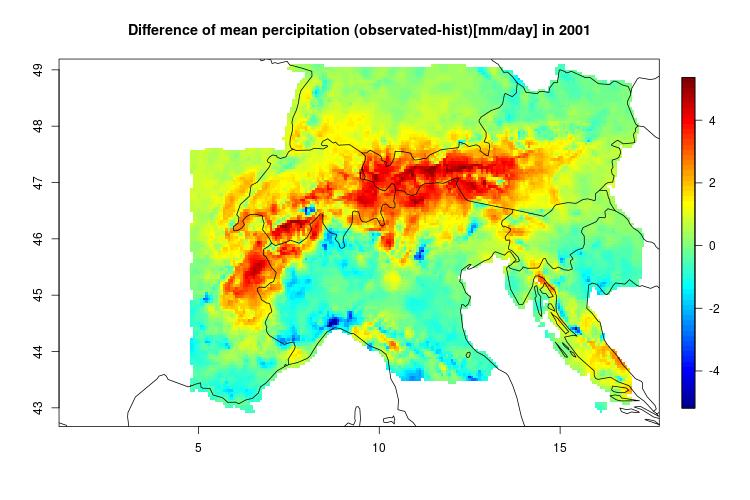
\includegraphics[width=\textwidth]{mean_n/2002dif_mprs_hist-obs.jpg}
			\caption{Historical, EUR-11}
			\label{fig:dif_mean_2002:eur11_hist}
		\end{subfigure}
		\begin{subfigure}{0.49\textwidth}
			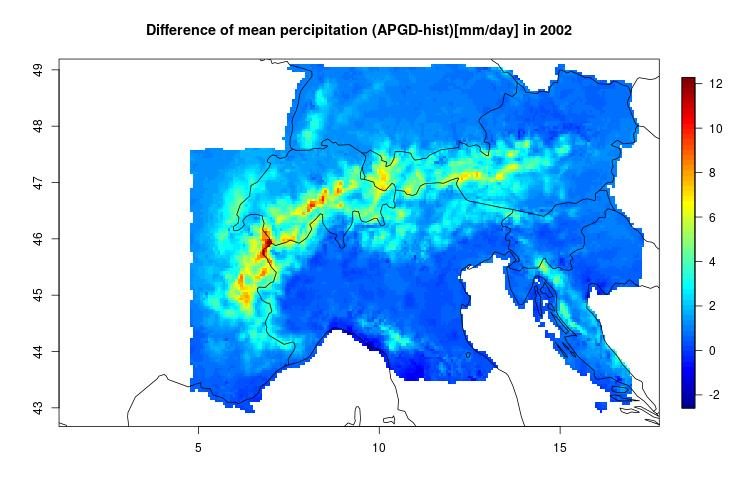
\includegraphics[width=\textwidth]{mean_n/2002dif_mprs_alp3hist-apgd.jpg}
			\caption{Historical, ALP-3}
			\label{fig:dif_mean_2002:alp3_hist}
		\end{subfigure}
		\begin{subfigure}{0.45\textwidth}
			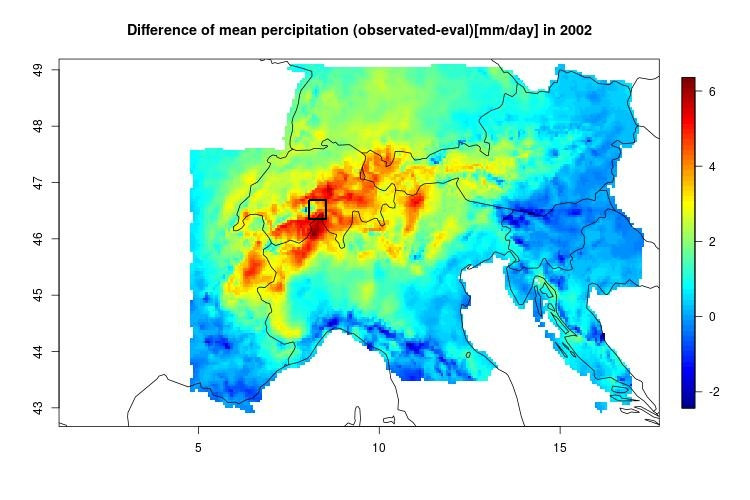
\includegraphics[width=\textwidth]{mean_n/2002dif_mprs_eval-obs.jpg}
			\caption{Evaluation, EUR-11}
			\label{fig:dif_mean_2002:eur11_eval}
		\end{subfigure}
		\begin{subfigure}{0.45\textwidth}
			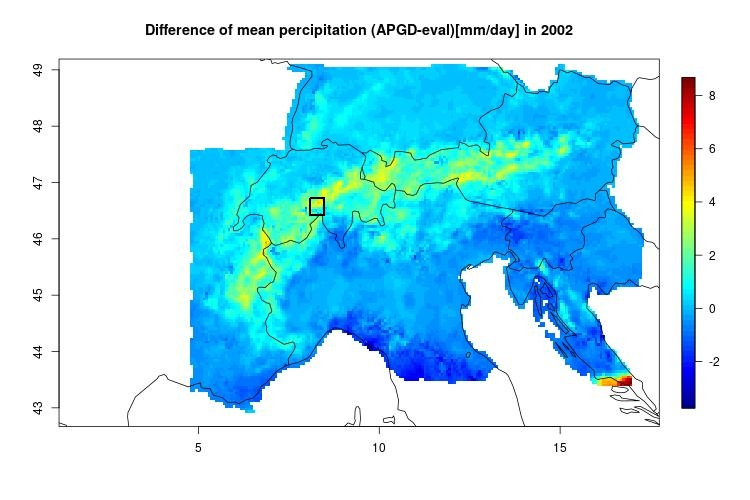
\includegraphics[width=\textwidth]{mean_n/2002dif_mprs_alp3eval-apgd.jpg}
			\caption{Evaluation, ALP-3}
			\label{fig:dif_mean_2002:alp3_eval}
		\end{subfigure}
	\caption{Differenzen des jährlichen Mittels über den Niederschlag im Jahr 2002}
	\label{fig:dif_mean_2002}
\end{figure}

Wie in den Grafiken bei Abb.\ref{fig:dif_mean_2002} zu erkennen ist bleibt in einem gewissen Bereich die Abweichungen über alle Datensätze am größten. Deshalb wurde dieser in Folge gesondert betrachtet. Der Bereich wurde in den Abbildungen gekennzeichnet.\\
Diese gekennzeichnete Fläche wurde aus allen Datensätzen ausgeschnitten und im Jahr 2002 über dessen Fläche gemittelt, somit ergab sich aus dem Rechteck ein Mittelwert für jeden Tag für jeden Datensatz. Von diesen Werten wurden dann die ebenfalls Flächen-gemittelten Beobachtungsdaten (APGD) abgezogen und im Diagramm in Abb.\ref{fig:diff_2002} gegen die Zeit aufgetragen.\\
\begin{figure}[h]
	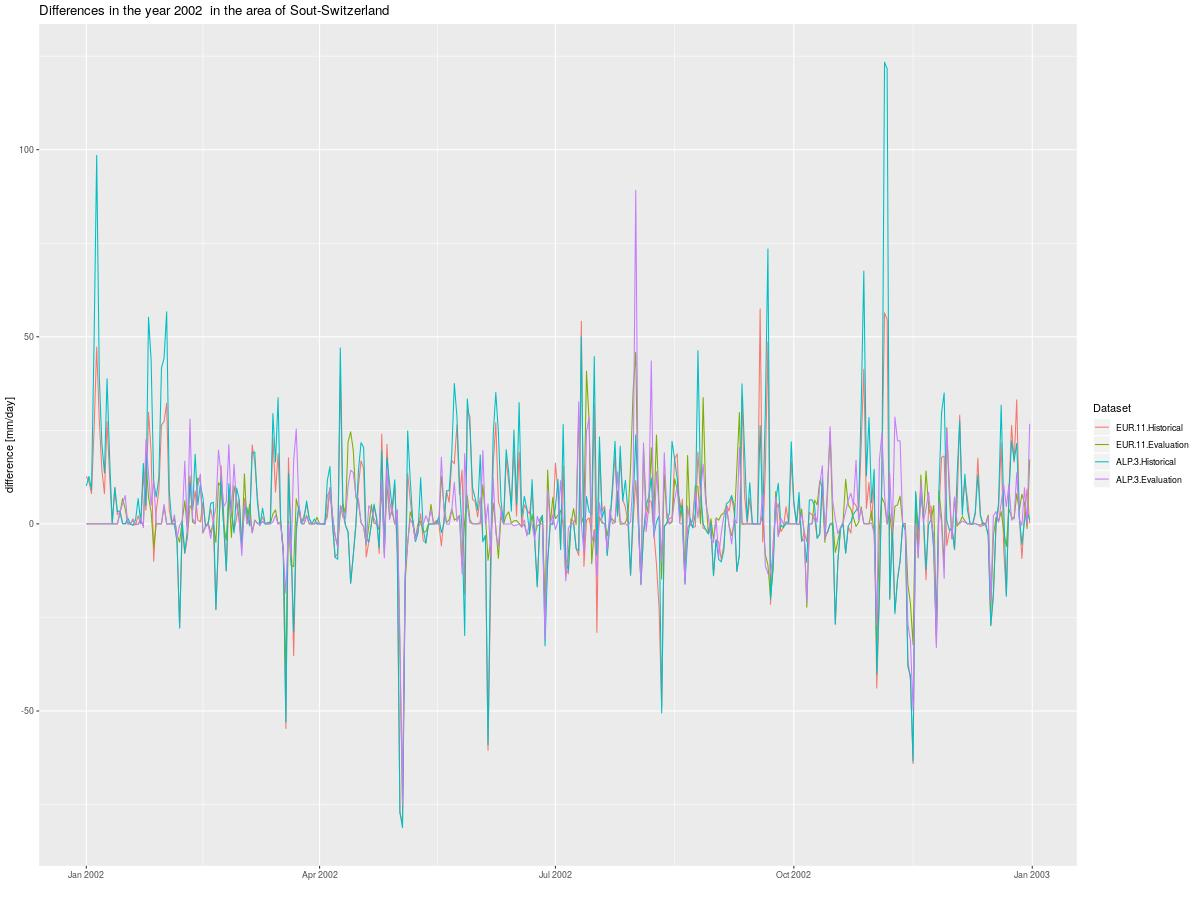
\includegraphics[width=0.95\textwidth]{mean_n/differences_2002.jpg}
	\caption{Die Differenzen für den in der Abb. \ref{fig:dif_mean_2002} gekennzeichneten Bereich im Jahr 2002. Es muss beachtet werden, dass hier die tägliche Inkonsistenz betrachtet wird, dies ist nicht ein Fehler des Modells.}
	\label{fig:diff_2002}
\end{figure}\\
Man sieht in Abb.\ref{fig:diff_2002}, dass die Abweichungen über das Jahr verteilt stark fluktuieren. Beachtenswert ist dabei, dass die Ausschläge der Kurven für den ALP-3 Datensatz deutlich größer und auffallend in das Positive verschoben sind. Die Kurvenform der beiden, Historical und Evaluation Datensätzen sind nahezu identisch, was auf Fehler in den Antriebsdaten zurückzuführen ist. Da die Ausschläge gemittelt über das ganze Gebiet (vgl. Abb.\ref{fig:mean_boxplots} und Abb.\ref{fig:mean_freq_plots}) für den ALP-3 Datensatz deutlich besser sind ist es in diesem gesondert betrachteten Gebiet wahrscheinlich zu einem Overfitting des Modells gekommen und die extremen Ausschläge sind Fluktuationen die daraus resultieren. Um die Ergebnisse der beiden RCM's EUR-11 und ALP-3 besser untersuchen zu können wurden die zwei Datensätze mit den größten Abweichungen (Historical aus EUR-11 und ALP-3) in Abb.\ref{fig:precip_2002} dargestellt.\\

\begin{figure}[b]
	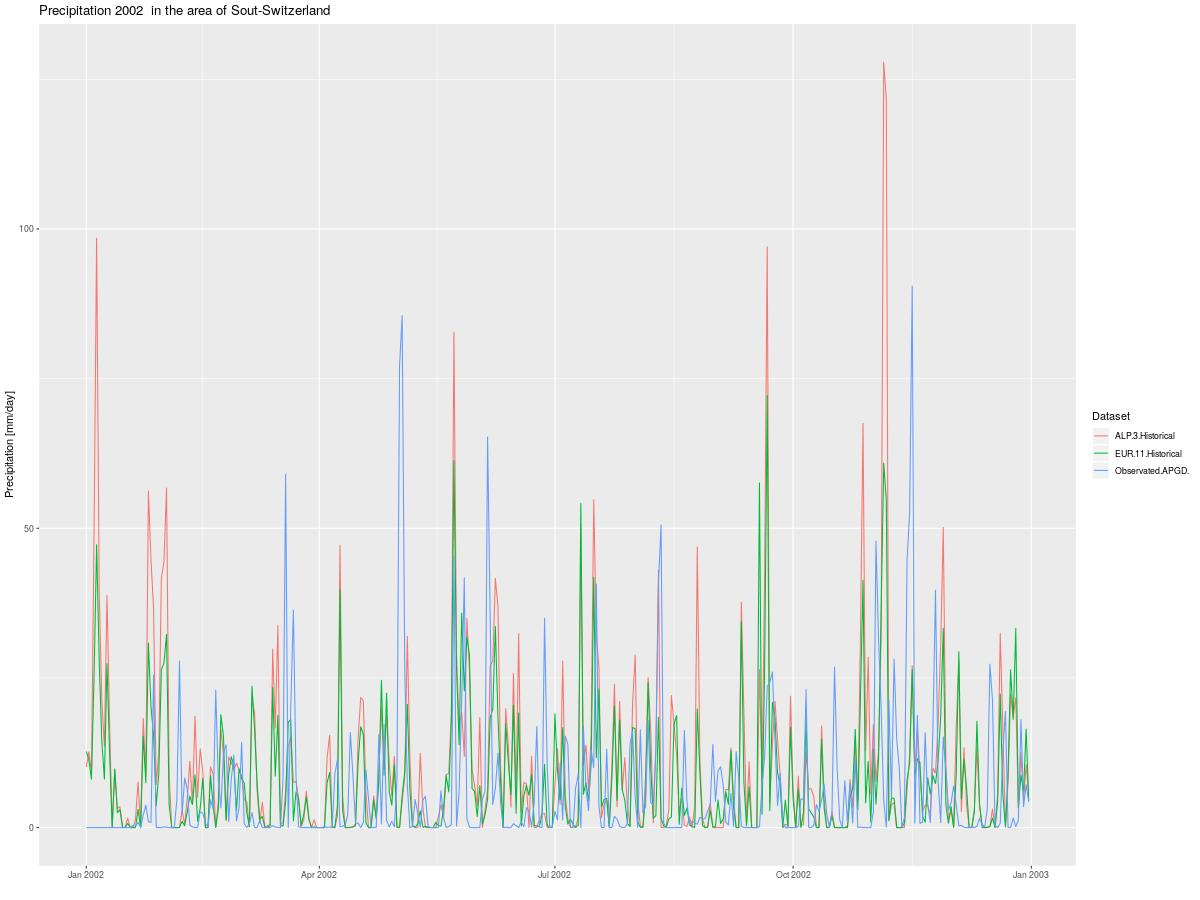
\includegraphics[width=0.90\textwidth]{mean_n/historical_2002.jpg}
	\caption{Niederschlag im Jahr 2002 für den in Abb.\ref{fig:dif_mean_2002} gekennzeichneten Bereich aus den Datensätzen Historical von ALP-3 bzw. EUR-11 gegen die Beobachtungsdaten aus APGD}
	\label{fig:precip_2002}
\end{figure}
\begin{figure}[b]
	\begin{subfigure}{0.49\textwidth}
		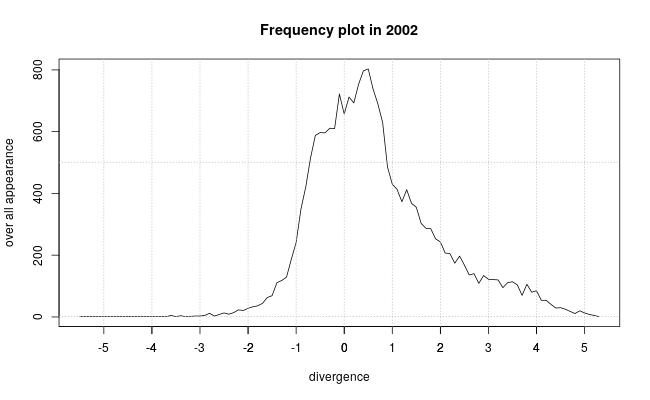
\includegraphics[width=\textwidth]{mean_n/2002frequenciesdif_mprs_hist-obs.jpg}
		\caption{EUR-11, Historical}
	\end{subfigure}
	\begin{subfigure}{0.49\textwidth}
		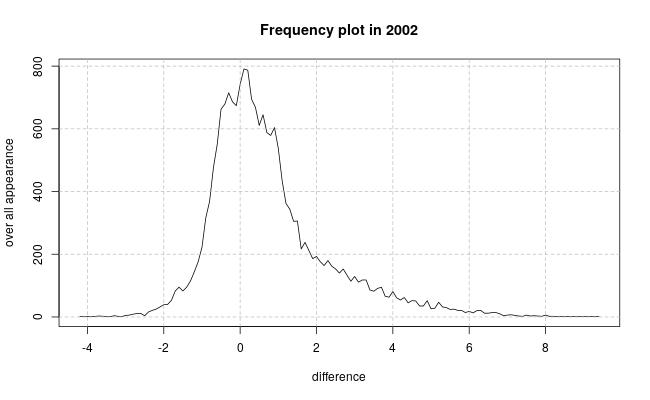
\includegraphics[width=\textwidth]{mean_n/2002frequenciesdif_mprs_alp3hist-apgd.jpg}
		\caption{ALP-3, Historical}
	\end{subfigure}
	\begin{subfigure}{0.49\textwidth}
		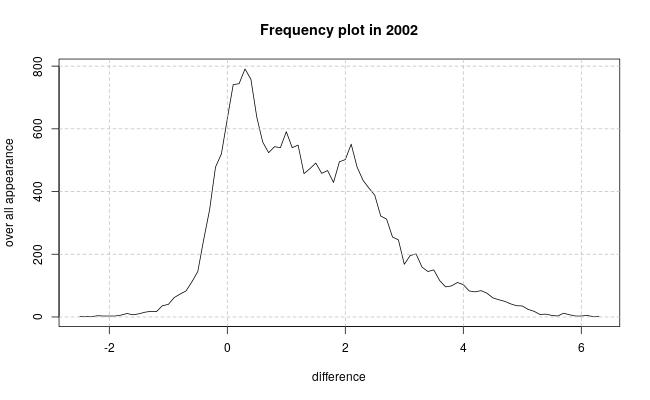
\includegraphics[width=\textwidth]{mean_n/2002frequenciesdif_mprs_eval-obs.jpg}
		\caption{EUR-11,Evaluation}
	\end{subfigure}
	\begin{subfigure}{0.49\textwidth}
		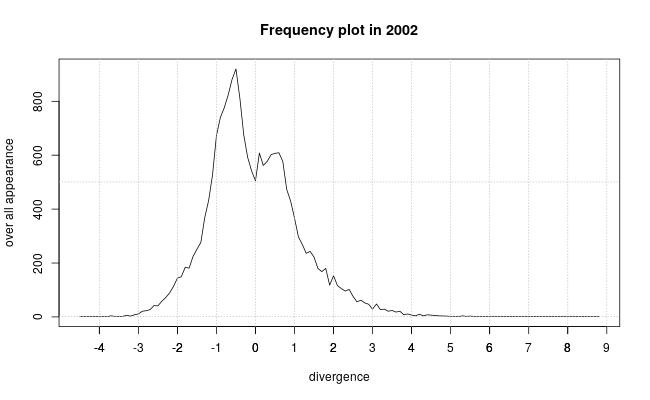
\includegraphics[width=\textwidth]{mean_n/2002frequenciesdif_mprs_alp3eval-apgd.jpg}
		\caption{ALP-3, Evaluation}
	\end{subfigure}
	\caption{Häufigkeit gewisser Abweichungen für das gemittelte Jahr 2002 in den beiden Historical - Datensätzen (betrachtetes Gebiet: \underline{gesamter} Alpenraum)}
	\label{fig:freq_2002}
\end{figure}

In der Abb. \ref{fig:precip_2002} liegen die im regionalen Klimamodell (ALP-3) die vorhergesagten Niederschlagsmengen für größere Niederschlagsmengen z.B. im Mai 2002 um einiges näher an den beobachteten Daten. Es werden jedoch auch manche Niederschlagsereignisse schlichtweg überschätzt, was sich dann im Gesamtbild schlecht auswirkt (vgl.\ref{fig:freq_2002}: die Kurve ist deutlich ins Positive verschoben.\\
Das Klimamodell welches die Konvektion nicht simuliert (EUR-11) scheint dauernd eine gewisse Fluktuation im Niederschlag zu errechnen, ohne gezielt Starkregenereignisse zu reproduzieren. Dies ist gut im Bereich April 2002 in der Abb. \ref{fig:precip_2002} zu erkennen: Die Fluktuationen scheinen gewissermaßen ständig aufzutreten. Das ist auf die Parametrisierung der Konvektion zurückzuführen. Da dadurch auch keine längeren Regenpausen vorkommen können, ist dies ein großes Manko in der Vorhersagekraft von diesen Modellen für die zukünftige Entwicklung des Klimas auf regionaler Ebene (siehe ''Bias Correction, Quantile Mapping, and Downscaling: Revisiting the Inflation Issue'' von D.Maraun \cite{biasMaraun}). \\
Das Konvektion-simulierende Klimamodell ALP-3 scheint besonders im Winter und im Herbst Niederschlagsextrema zu überschätzen. Im Sommer  bzw. Frühling stimmen die Daten relativ gut überein. Manche Extrema sind zwar zeitlich verschoben, jedoch muss bemerkt werden, dass die historischen Tage nichts mit den simulierten Tage im Klimamodell gemein haben, somit darf die zeitliche Verteilung nicht zu genau genommen werden. Sondern es muss eine gewisse Toleranz, wann ein Starkregenereignis eintritt mit-einberechnet werden.\\
\end{comment}
\section{Zusammenfassung}\label{sec:zusammenfassung_01}
Wie in diesem Kapitel gezeigt wurde, liegen die Abweichungen der Mittelwerte beider regionalen Klimamodell ähnlich verteilt vor. Dies kann darauf zurückgeführt werden, dass das feinere RCM CCLM5-0-9 in das gröber genested wurde. Die beiden Datensätze (ALP3 und EUR11) unterscheiden sich besonders in den Ausreißern (vgl. Abb \ref{fig:mean_boxplots}). Das feinere RCM hat viel stärkere maximale Abweichungen als das gröbere. Dies ist auf das noch mangelhafte Tuning des jüngeren und feineren Modells zurückzuführen.\\
Durch das Mitteln der Daten wurden die Extremniederschläge aus den Daten ''weggemittelt'' und da der Mittelwert des Niederschlags nicht das Klima einer Region beschreibt kann der Mittelwert nicht zur vollständigen Evaluation eines Modells herangezogen werden. Nichtsdestotrotz gibt der Mittelwert einen guten Aufschluss darüber, wo die größten Abweichungen herrschen (siehe Abbildung \ref{fig:mean_diff}). Will man eine einzelne Region über eine Jahreszeit oder auch die gesamte Zeitspanne genauer betrachten, steht man vor dem Problem, dass die simulierten Tage nicht direkt mit den historischen Tagen in Verbindung gebracht werden dürfen(vgl. Kapitel \ref{chap:modells}). Um nun diese tägliche Inkonsistenz aus der Evaluierung außenvorzulassen, soll im nächsten Kapitel auf die alljährlichen Extremniederschläge über das 99.Quantil eingegangen werden, wodurch diese Inkonsistenz in den Kalendertagen umgangen wird: Es wird nicht der Tag X in den Beobachtungsdaten mit dem Tag X in den Modelldaten verglichen, sondern der Tag mit dem höchsten Niederschlag bzw. dem 99.Quantil des Niederschlag in beiden Datensätzen.
\section{R-Code}
\begin{lstlisting}[language=R]
	observation <- stackAPGD(getAPGD())
	mean_observations<-getAnnualMeanObs(observation)
	mean_mean_observations<-calc(mean_observations, fun=mean)
	eval_eur11 <- stackSim(getEUR11regridded_eval_pr(), varname = "pr", factor = 3600*24) # factor for the precipitation-unit
	mean_eval_eur11<-getAnnualMeanSim(eval_eur11) # calculates the annual mean and places it in a raster (=>10years==10layers)
	mean_mean_eval_eur11 <- calc(mean_eval_eur11, fun=mean) #calculate the mean over all years
	extent(mean_mean_observations)<-extent(mean_mean_eval_eur11) # for better representation
	dif_mean_eval_eur11<-overlay(mean_mean_eval_eur11, mean_mean_observations,fun=function(x,y){return((x - y))}) #subtract each grid-cell
\end{lstlisting}
Ein Ausschnitt des Codes, der für die Berechnungen des Mittelwertes und der Differenzen verwendet wurde. Die Funktionen getAPGD() und getEUR11regrid\_eval\_pr() liefern eine liste der Dateien mit den Daten zurück. Die beiden Funktionen stackSim() und stackAPGD() legen die Daten in eine Liste aus rastern ab. Danach wird über die einzelnen Elemente der Liste der Mittelwert und in Folge der Mittelwert aller Mittelwerte berechnet (stets für jede Zelle einzeln). Diese Mittelwerte werden voneinander abgezogen (Modell - Beobachtung).